\documentclass[10pt,]{article}
\usepackage[left=1in,top=1in,right=1in,bottom=1in]{geometry}
\newcommand*{\authorfont}{\fontfamily{phv}\selectfont}
\usepackage[]{mathpazo}


  \usepackage[T1]{fontenc}
  \usepackage[utf8]{inputenc}



\usepackage{abstract}
\renewcommand{\abstractname}{}    % clear the title
\renewcommand{\absnamepos}{empty} % originally center

\renewenvironment{abstract}
 {{%
    \setlength{\leftmargin}{0mm}
    \setlength{\rightmargin}{\leftmargin}%
  }%
  \relax}
 {\endlist}

\makeatletter
\def\@maketitle{%
  \newpage
%  \null
%  \vskip 2em%
%  \begin{center}%
  \let \footnote \thanks
    {\fontsize{18}{20}\selectfont\raggedright  \setlength{\parindent}{0pt} \@title \par}%
}
%\fi
\makeatother




\setcounter{secnumdepth}{0}


\usepackage{graphicx}
% We will generate all images so they have a width \maxwidth. This means
% that they will get their normal width if they fit onto the page, but
% are scaled down if they would overflow the margins.
\makeatletter
\def\maxwidth{\ifdim\Gin@nat@width>\linewidth\linewidth
\else\Gin@nat@width\fi}
\makeatother
\let\Oldincludegraphics\includegraphics
\renewcommand{\includegraphics}[1]{\Oldincludegraphics[width=\maxwidth]{#1}}

\title{Assesing Health Care Coverage and Access Utilizing the National Health
Interview Survey  }



\author{\Large John Diego\vspace{0.05in} \newline\normalsize\emph{University of Washington}   \and \Large Warren Wakuzawa\vspace{0.05in} \newline\normalsize\emph{University of Washington}   \and \Large Adrian Santiago\vspace{0.05in} \newline\normalsize\emph{University of Washington}  }


\date{}

\usepackage{titlesec}

\titleformat*{\section}{\normalsize\bfseries}
\titleformat*{\subsection}{\normalsize\itshape}
\titleformat*{\subsubsection}{\normalsize\itshape}
\titleformat*{\paragraph}{\normalsize\itshape}
\titleformat*{\subparagraph}{\normalsize\itshape}





\newtheorem{hypothesis}{Hypothesis}
\usepackage{setspace}

\makeatletter
\@ifpackageloaded{hyperref}{}{%
\ifxetex
  \usepackage[setpagesize=false, % page size defined by xetex
              unicode=false, % unicode breaks when used with xetex
              xetex]{hyperref}
\else
  \usepackage[unicode=true]{hyperref}
\fi
}
\@ifpackageloaded{color}{
    \PassOptionsToPackage{usenames,dvipsnames}{color}
}{%
    \usepackage[usenames,dvipsnames]{color}
}
\makeatother
\hypersetup{breaklinks=true,
            bookmarks=true,
            pdfauthor={John Diego (University of Washington) and Warren Wakuzawa (University of Washington) and Adrian Santiago (University of Washington)},
             pdfkeywords = {healthcare, NHIS, ACA, medicaid, medicare},  
            pdftitle={Assesing Health Care Coverage and Access Utilizing the National Health
Interview Survey},
            colorlinks=true,
            citecolor=blue,
            urlcolor=blue,
            linkcolor=magenta,
            pdfborder={0 0 0}}
\urlstyle{same}  % don't use monospace font for urls



\begin{document}
	
% \pagenumbering{arabic}% resets `page` counter to 1 
%
% \maketitle

{% \usefont{T1}{pnc}{m}{n}
\setlength{\parindent}{0pt}
\thispagestyle{plain}
{\fontsize{18}{20}\selectfont\raggedright 
\maketitle  % title \par  

}

{
   \vskip 13.5pt\relax \normalsize\fontsize{11}{12} 
\textbf{\authorfont John Diego} \hskip 15pt \emph{\small University of Washington}   \par \textbf{\authorfont Warren Wakuzawa} \hskip 15pt \emph{\small University of Washington}   \par \textbf{\authorfont Adrian Santiago} \hskip 15pt \emph{\small University of Washington}   

}

}







\begin{abstract}

    \hbox{\vrule height .2pt width 39.14pc}

    \vskip 8.5pt % \small 

\noindent The National Health Interview Survey (NHIS) is the nation's largest
in-person household health survey. It has been conducted annually since
1957 by the National Center for Health Statistics (NCHS), which is a
part of the Centers for Disease Control and Prevention (CDC). A broad
range of topics are covered but we will specifically focus on healthcare
access and expenditure across a multitude of factors such as employer
information, race, and academic background.


\vskip 8.5pt \noindent \emph{Keywords}: healthcare, NHIS, ACA, medicaid, medicare \par

    \hbox{\vrule height .2pt width 39.14pc}



\end{abstract}


\vskip 6.5pt

\noindent  \section{INTRODUCTION}\label{introduction}

The Patient Protection and Affordable Care Act (PPACA), commonly
shortened to the Affordable Care Act (ACA) and nicknamed Obamacare, is
one of the most important healthcare legislature, creating a significant
impact on the US Health care system. However, with the arrival of
President Trump in the Oval Office, and with the ACA repeal now
underway, some speculate huge consequences such as
\href{https://www.washingtonpost.com/posteverything/wp/2017/01/23/repealing-the-affordable-care-act-will-kill-more-than-43000-people-annually/?utm_term=.a2fbb24cd075}{increased
death rates}. In light of these recent events, it is important that we
take a look at the current state of our healthcare system and question
whether it is failing or not.

The purpose of this paper is to assess healthcare coverage and access
across a multitude of factors. We will specifically look at three
aspects of health care - the first aspect is the relationship between
educational attainment and access to medical insurance, the second is an
overall look at the population and health care coverage, and the final
exploration covers healthcare expenditure over the years.

\section{METHODOLOGY}\label{methodology}

To answer the questions we layed out, we use data provided from the NHIS
survey. We used various subsets of the survey data, depending on the
specific question being analyzed.

\subsection{\texorpdfstring{\textbf{Educational Attainment Vs Healthcare
Access}}{Educational Attainment Vs Healthcare Access}}\label{educational-attainment-vs-healthcare-access}

To answer the question, \emph{``Does higher educational attainment cause
greater chance of acquiring medical insurance?''}, we filtered the
dataset, only looking a three specific variables, the \emph{highest
educational attainment}, \emph{health insurance coeverage}, and
\emph{health insurance offered at workplace}.

Because the dataset was so large, it was difficult to manage and
processing the data was time-consuming. In order to fully combat this,
we used the dplyr package in order to modify the dataset we would be
using in such a way that only incorporated the columns we needed to
address the question at hand. After, we then filtered the data so that
we would have only the information we needed to answer the questions,
while weeding out ``empty'' data such as ``not ascertained,'' ``didn't
know,'' as well as ``refused.'' When we were certain of the dataset we
needed that only contained relevant information to our questions, we
then utilized the ggplot2 R package in order to create well-labeled
graphs that visually summarized our results. From the graphs, we were
able to draw reasonable conclusions and generate an analysis of why the
data was shaped in the particular way it was.

\subsection{\texorpdfstring{\textbf{Health Care
Access}}{Health Care Access}}\label{health-care-access}

In respects to the National Health Interview Survey, we wanted to
research what percentage of the population had healthcare coverage. We
used the ``NOTCOV'' column of the survey to retrieve the amount of
individuals that had coverage and those who did not have healthcare
coverage. We do want to mention that there was a total of 1102
individual that responded with ``Don't know''. WE made the decision to
exclude these individuals from our data since they do not represent your
targeted population.

When comparing just the proportions of those who had healthcare coverage
to those who lacked coverage, there was a clear transformation. Only
10.23\% of the individuals that participated in this survey did not have
healthcare coverage. While 89.76\% of these individuals did have
coverage.

\subsection{\texorpdfstring{\textbf{Health Care
Expedentiture}}{Health Care Expedentiture}}\label{health-care-expedentiture}

To gain a general outlook on the healthcare system, one way of looking
at it is through the perspective of expenditures. Specifically the
question we wanted to explore is, \emph{``How has the amount of money
spent for medical care changed over the years?''} One specific variable
that was counted for from the survey was \emph{``Amount family spent for
medical care, past 12 months''}. To see this distribution, data from the
2005 to 2015 NHIS surveys was used (N=1,033,155). We then filtered the
data further down to those who responded back to the question (N =
994,797). The distribution of health expenditure over the years can be
seen in the graph below.

This independent variable only provides a rough estimate on the family's
expenditure on medical care, but is still relevant since interviewers
directed respondents to exclude the insurance premiums, over-the-counter
drugs, and any costs for which they expected to be reimbursed.

To make calculations on the greater population, we used the calculated
weight and strata within the provided by those who constructed the NHIS
dataset. According to the \href{https://ihis.ipums.org/}{codebook}, the
\emph{sample weight} was calculated using ``adjustments for age,
race/ethnicity, and sex using the Census Bureau's population control
totals'', while \emph{strata} was represents ``the impact of the sample
design stratification on the estimates of variance and standard
errors.'' A \textbf{stratified random sampling} was implemented to
calculate the weighted proportions of people who spend X amount for
health insurance, X being multiple levels of range of money spent.

\section{RESULTS}\label{results}

\subsection{\texorpdfstring{\textbf{Plots}}{Plots}}\label{plots}

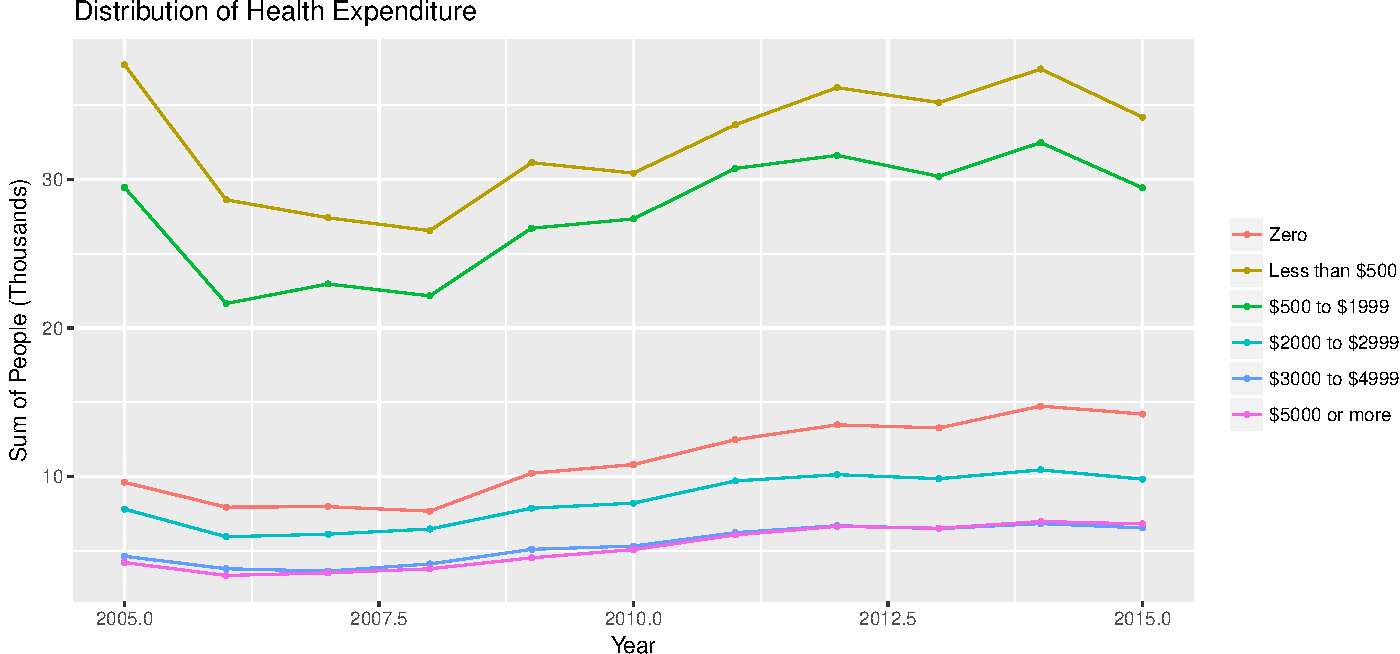
\includegraphics{paper_files/figure-latex/expenddistribution-1.pdf}
\textbf{Figure 1. Expenditure Distribution over Time}

\smallskip

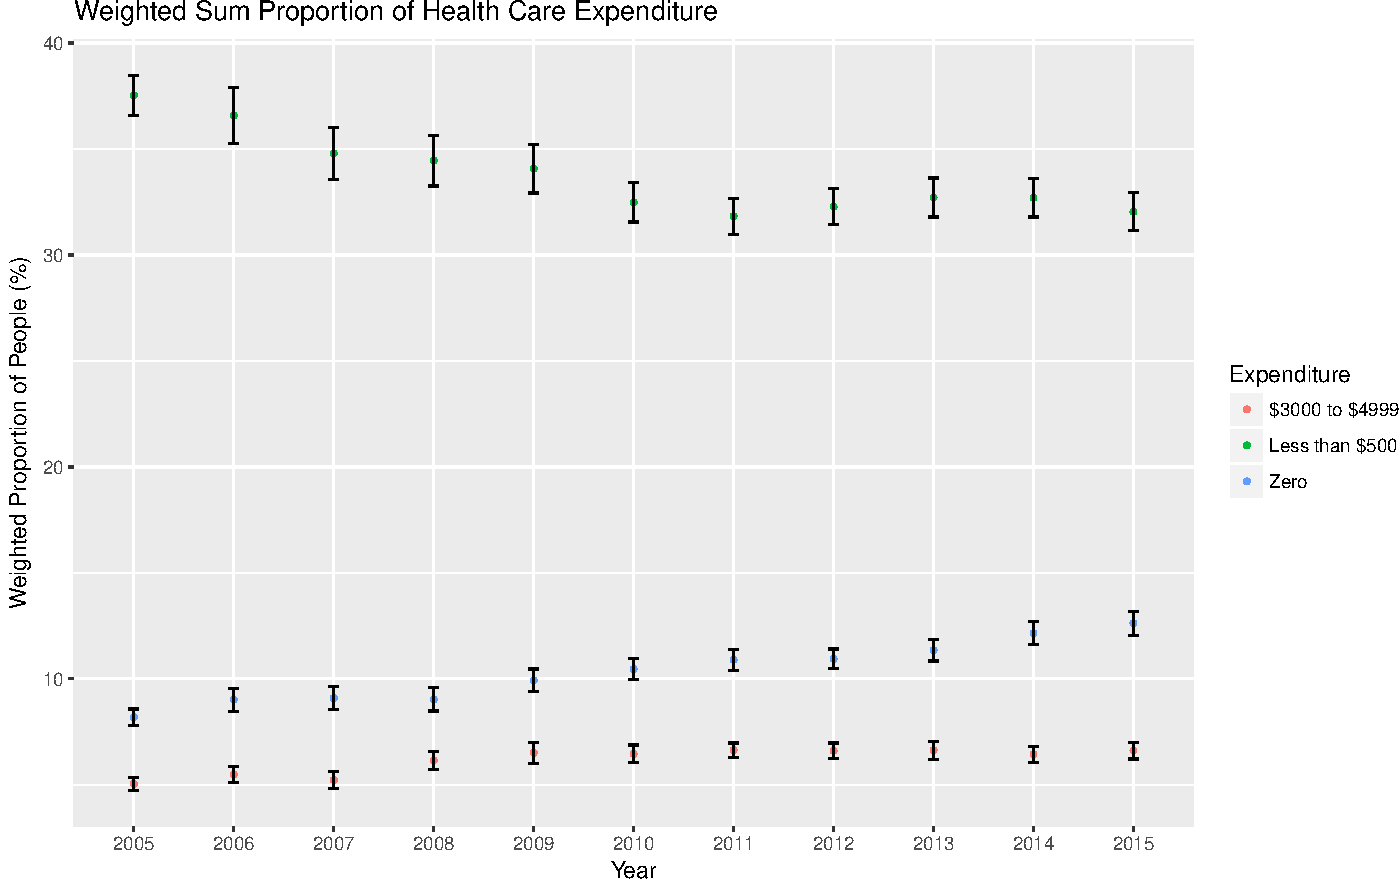
\includegraphics{paper_files/figure-latex/weightedexpendproportion-1.pdf}
\textbf{Figure 2. Expenditure Distribution over Time (Weighted)}

\smallskip

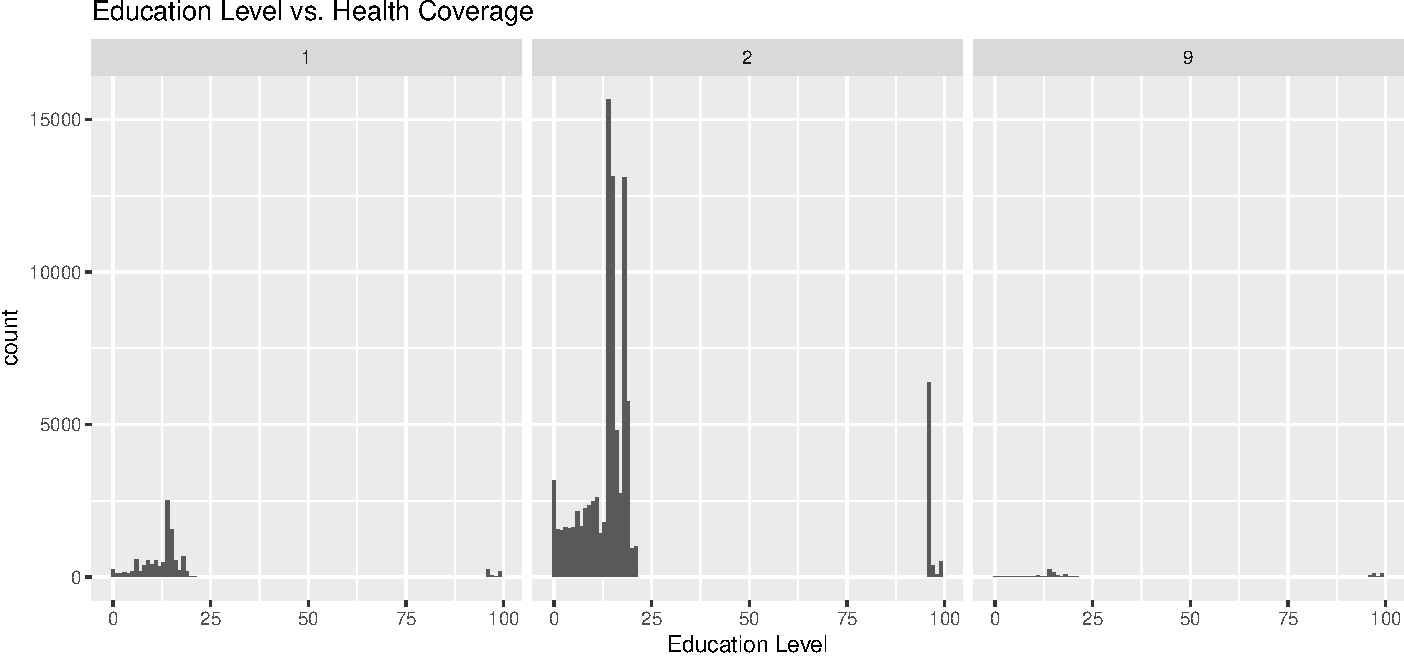
\includegraphics{paper_files/figure-latex/healthcovereduattainment-1.pdf}
\textbf{Figure 3. Distribution of Health Coverage per Education Level}

\smallskip

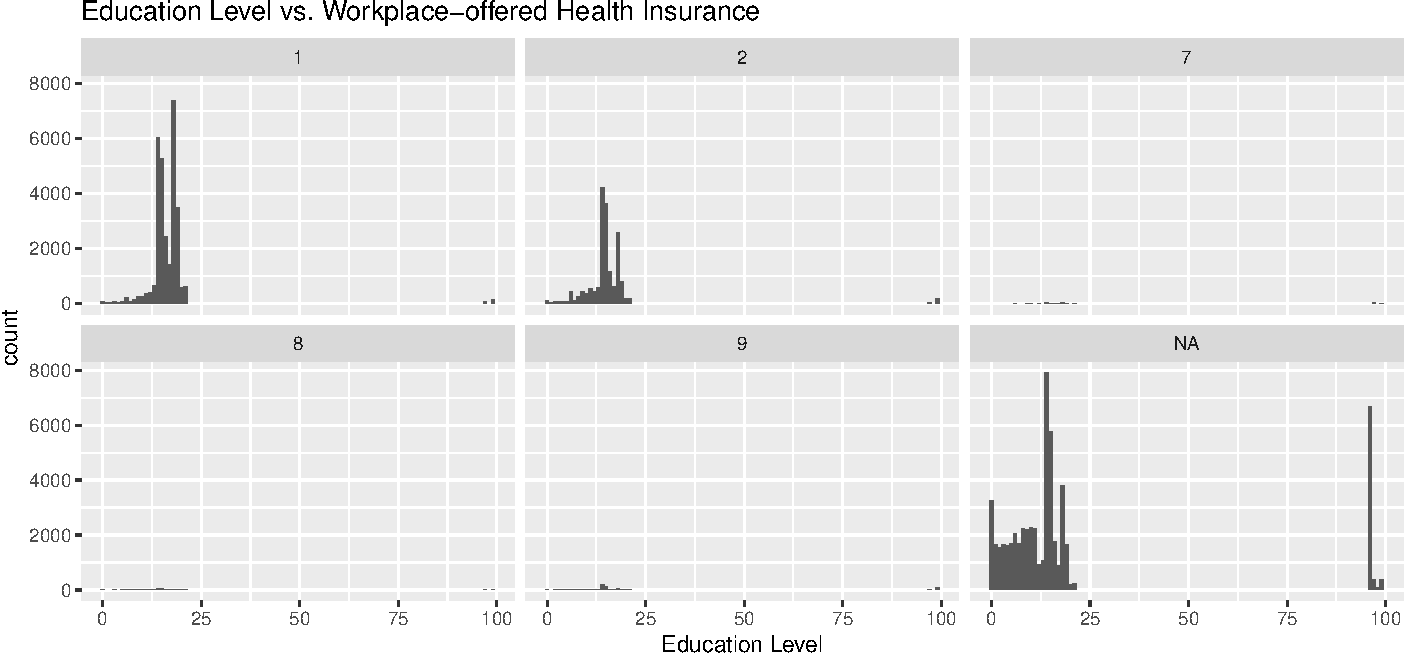
\includegraphics{paper_files/figure-latex/workhealthinsuranceeduattainment-1.pdf}
\textbf{Figure 4. Educational Attainment vs.~Workplace-offered Health
Insurance}

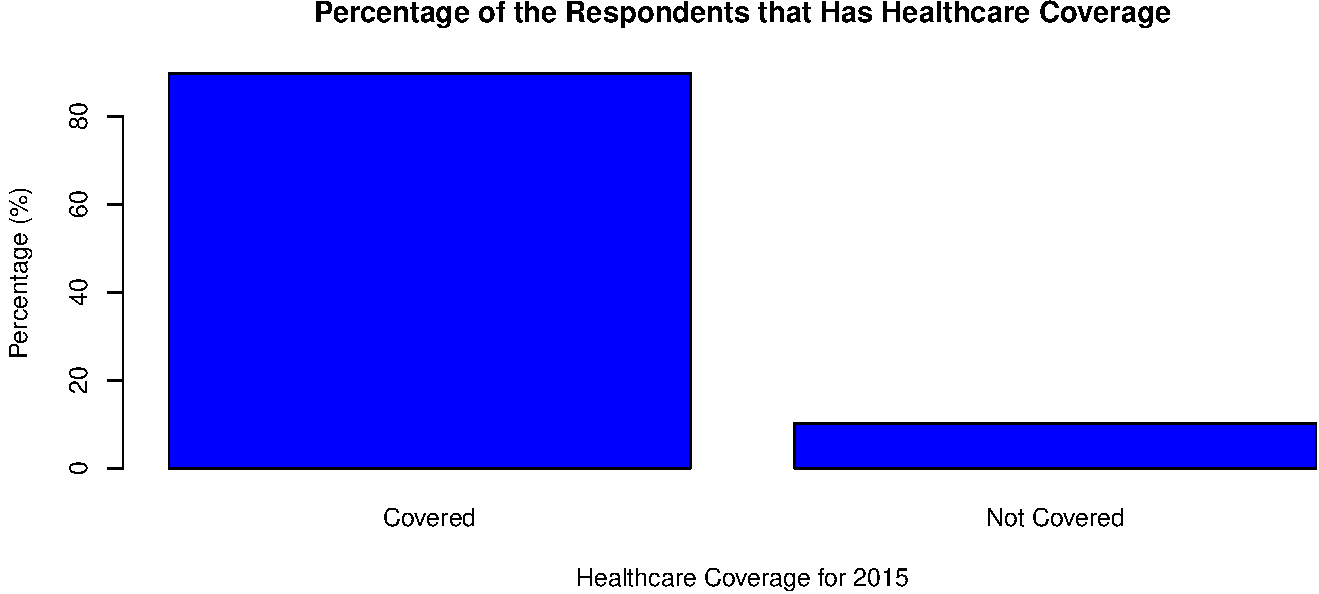
\includegraphics{paper_files/figure-latex/hi2015-1.pdf}

\textbf{Figure 5. Percentage of the Respondents that Has Healthcare
Coverage}

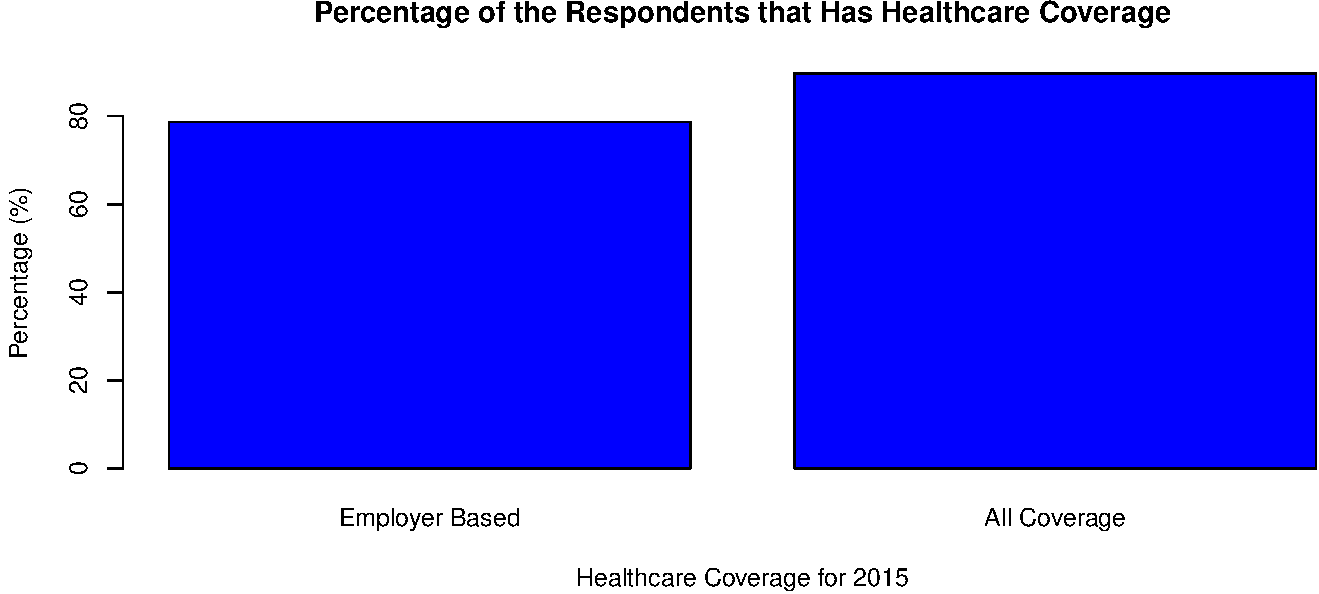
\includegraphics{paper_files/figure-latex/hi2015employer-1.pdf}
\textbf{Figure 6. Percentage of the Respondents that Has Healthcare
Coverage}

\section{DISCUSSION}\label{discussion}

\subsection{\texorpdfstring{\textbf{Educational Attainment Vs Healthcare
Access}}{Educational Attainment Vs Healthcare Access}}\label{educational-attainment-vs-healthcare-access-1}

The first graph that we see here represents whether or not an individual
obtained health coverage based on their education level. Immediately, we
see that the number 2 subgraph contains a lot more results than the
number 1 subgraph, which indicates that there were more people who
received health coverage than did not. Under the number 1 subgraph, we
see the varying number of people who did not receive health coverage
given their level of education. There appears to be a notable peak at
the number 14 which is indicative of those who have completed up to a
high school diploma. A second notable peak is at the number 15 which
represents those who have attended college but had not received a
degree. Such might be the case because most people finish school up
until high school and also attend college, so it would make sense that
the bulk of the sample surveyed would reside in that educational
attainment categories. It would furthermore make sense that they did not
receive health coverage because nowadays, people obtain health/medical
insurance from their workplaces since getting these plans on an
individual basis is a lot more expensive. Those who did not finish
college or only obtained a high school diploma might have not been able
to get the best occupation due to their lack of education and skills in
the workforce, which affected their ability to get health coverage from
their employer.

In the number 2 subgraph, we see three notable peaks--one at the
x-coordinate values 14, 15, and 18. These peaks correspond to the bulk
of those who received health/medical insurance given that they either
graduated high school, went to college but did not get a degree, or got
a Bachelor's degree. What is interesting about this is that there were a
lot of people who did not AND did get health coverage given that they
graduated from high school or went to college but did not get a degree.
This might reveal to us that even with a high school degree it is
possible to get a steady job that includes medical/health insurance
coverage. However, analyzing the data further, it makes sense that a lot
of people who received health coverage received at least a Bachelor's
degree, because that level of education makes it a lot easier to get
jobs that pay well and include a lot of benefits such as medical
insurance.

The second graph we are looking at compares educational attainment with
whether or not a person received health insurance from their workplace.
The number 1 subgraph represents the count of people who did
\emph{receive health insurance at their workplace} given their highest
level of educational attainment, while number 2 subgraph represents the
count of people who \emph{did not receive health insurance at work}
given their highest level of educational attainment. Again, in both
graphs, x-coordinate values 14, 15, and 18, corresponding to having
graduated high school, attending college without getting a degree, and
getting a bachelor's degree respectively, are the most prominent peaks
in the graph. This is due to the fact that most people finish at least
up until high school, attend college at some point and realize that it
wasn't for them, or obtain their bachelor's degree. Very \emph{few}
people quit grade school in the middle of it and very few people get a
higher education such as a master's or doctoral degree, which is why the
sample count is so low at those other values. Based on the number 1
subgraph however, we see that the most people who got health insurance
from their workplace are those who graduated with a Bachelor's degree.
This reveals the importance of obtaining a Bachelor's degree when
getting a job. Other interesting points of analysis are that more high
school graduates received workplace-offered health insurance than those
who attended college but did not get a degree. One reasoning behind this
is that those who did not receive a degree from college might have been
those who quit in order to pursue their own businesses, and therefore
did not work for an existing corporation that would have otherwise
offered them health insurance. The number 2 subgraph shows that high
school graduates were the least likely to receive health insurance from
their workplace, which again points back to the fact that they probably
weren't able to get a great enough job that offered them benefits such
as health insurance. Most decent jobs nowadays require people to have at
least a bachelor's degree. The lowest of the three peaks, though, are
those who got a bachelor's degree, and it shows that with a higher level
of education, you will have a \emph{better} chance of getting a job with
better benefits.

ODDS RATIO: 1.19 / 3.66 = \textbf{0.33} The odds of getting coverage
being a high school grad is 0.33 times higher than the odds of getting
coverage having a bachelor's degree.

\subsection{\texorpdfstring{\textbf{Health Care
Access}}{Health Care Access}}\label{health-care-access-1}

A huge discussions these recent weeks has been Obama care. Some view it
was a total disaster while others suggest that it works but it is not
perfect. Our president has spoken that this plan is terrible and this
inspired us to consider the what a reality would be like if there was no
more Obama care. As a group we believed that without government help,
individuals would have to resort to other sorts of health care plans. We
decided to focus on employers to study if there is any significant
correlation between employers and health care coverage. We do have to
note that this information lacked the participation from 42728
individuals. This number was subtracted from the group that did
responded as we were interested in the population that did have some
sort of coverage.

As our prior graph indicates, about 89.76\% of the surveyed population
expressed some sort of healthcare coverage. Out of this population we
calculated that 78.69\% of population that has some sort of healthcare
coverage attains it through an employer. This is only about a 11.07\%
difference suggesting that the way more people get their healthcare
coverage through their workforce. However we did not count those
individuals who obtained coverage through their own self-employed
business, a union, or even those who were uncertain about their
response.

After analyzing these findings, it is our suggestion that there is some
relationship between employers and a person's' health care coverage. But
must point out that it is not very clear to understand how strong this
correlation is or to even identify in what specific ways these aspects
have an influence on each other. The 11\% difference does portray the
idea that everyone is obtaining healthcare coverage from their
employers. But it is crucial to realize that the portion that missed
this question represents, in quantity, consists of more than half the
population that did decide to answer. This great lack of representation
from the population is too big to consider a strong and clear
correlation between employers and health care coverage.

\subsection{\texorpdfstring{\textbf{Health Care
Expedentiture}}{Health Care Expedentiture}}\label{health-care-expedentiture-1}

For the chart concerning health care expenditure (Figure 2), We can see
the proportion of people who spent a specific level of money on health
insurance, whether it be zero,less than 500\$, or the other levels. For
example, we see that the largest proportion of people mostly spent less
than 500 dollars through out time, with atleast more than 30\% given any
year. Specifically, for 2005, 37.5\% percent of the population
\emph{spent less than 500 dollars}, but for 2015, it went down to
32.04\%. For the people \emph{spending no money} on health insurance,
this proportion mostly stayed between 8\% to 12\% over the years, with a
positive increase over time. Meanwhile, The proportion of people
\emph{spending between 3000 to 4000 dollars} doesn't have a linear
change over time like the other levels of expedenture. This proportion
stayed between 5\% and 6\% over time. Showing no linear change for
\emph{spending between 3000 to 4000 dollars} can be interpreted as a
positive income, since that means the proportion of the population
spending money on health insurance are not seeing an increase of
expenditure. One would expect that with the introduction of the
Affordable Care Act in 2010, which promised reducing health care costs,
the amount of money people are spending on health care would decrease.
These expectations turned out to be true, since the graph reflects a
positive rate of change for people spending no money on health
insurance, and negative rate of change for people spending less than 500
dollars.

\section{RELATED WORK}\label{related-work}

Previous projects have been done that measured trends in health
insurance coverage over the course of time. The report was done by the
National Center for Health Statistics (NCHS), and presents the selected
estimates for health insurance coverage among the civilian
noninstitutionalized U.S. population based on data from 2015 National
Health Interview Survey (NHIS), as well as comparable estimates from the
NHIS 2010-2014 surveys. From their results, they were able to determine
that the trends displayed an overall increase in the population that had
health insurance coverage in comparison to previous years. They then
observe short term trends by age, poverty status, as well as race and
ethnicity to provide a deeper insight of health insurance coverages, and
what might be influencing access to them.

\section{CONLUSION}\label{conlusion}

Our motivation to focus on healthcare was influenced from our class
discussions, guest speakers, and even or own personal experiences as
healthcare beneficiaries. We observe how the life of other individuals
are impacted by the opportunities to attain healthcare coverage. Through
our research project studied how health expenditure changed from
2005-2015 for individuals. Our findings help support that idea
individuals are mostly spending about less than five-hundred dollars per
year on medical charges. This information could be helpful to help
develop better health care options to target this population, as they
seem to represent a bigger portion of those who spend between
five-hundred to roughly five-thousand dollars per year.

Another finding of our research consisted of how of an impact did
education attainment have on healthcare access. One point of interest in
the educational system was high school. High school was a point that
indicated a change in healthcare accessibility. Those who went to pursue
higher education were observed to attain their coverage through their
workforce. This is something that differs from the idea that higher
education leads to more money which ultimately implies that you access
for healthcare coverage from your own earnings. It is interesting to
realize that the workforce could influence a person access to
healthcare.

Our last section of research consisted of the overall population and how
the proportions of healthcare coverage can differ. We realize that the
proportion of those who have some sort of healthcare coverage is larger
than the proportion of those who lack coverage. This, in our
perspective, is a positive finding as it is an indicator that more
people have access to healthcare. A final suggestion of our study is
that we hope to gain more information on the process of government's
funding. To be more specific we want to gain information on the exact
journey that government funds travel. We wish to know how certain
policies contribute to the healthcare funding of diverse organizations.
Our hopes to to find where government funding is increasing the
accessibility of healthcare coverage for any individual that wished to
attain it.

\section{REFERENCES}\label{references}

\begin{enumerate}
\def\labelenumi{\arabic{enumi}.}
\item
  IPUMS Health Surveys. Retrieved February 27, 2017 from
  \url{https://ihis.ipums.org/ihis/index.shtml}
\item
  David Himmelstein,Steffie Woolhandler. January 23, 2017. Repealing the
  Affordable Care Act will kill more than 43,000 people annually.
  Retrieved March 6, 2017 from
  \url{https://www.washingtonpost.com/posteverything/wp/2017/01/23/repealing-the-affordable-care-act-will-kill-more-than-43000-people-annually/?utm_term}=.a2fbb24cd075
\item
  Robin A. Cohen. May 2016. Health Insurance Coverage: Early Release of
  Estimates From the National Health Interview Survey, 2015. Retrieved
  March 2, 2017 from
  \url{https://www.cdc.gov/nchs/data/nhis/earlyrelease/insur201605.pdf}
\end{enumerate}
\newpage
\singlespacing 
\end{document}svm